
% This LaTeX was auto-generated from MATLAB code.
% To make changes, update the MATLAB code and republish this document.

\documentclass{article}
\usepackage{graphicx}
\usepackage{color}

\sloppy
\definecolor{lightgray}{gray}{0.5}
\setlength{\parindent}{0pt}

\begin{document}

    
    
\section*{APPM 2360 Project 2}


\subsection*{Contents}

\begin{itemize}
\setlength{\itemsep}{-1ex}
   \item 2.1 Questions
   \item 2
   \item 3
   \item 4
   \item 3.1 Questions
   \item 1
   \item 2
   \item 4
   \item 5
   \item 4.1 questions
   \item 1
   \item 2
   \item 3
   \item 4
   \item 5
\end{itemize}


\subsection*{2.1 Questions}

\begin{verbatim}
close all
clear all
\end{verbatim}


\subsection*{2}

\begin{verbatim}
Ps = 0.7;
Pe = 0.4;
Pi = 1;
Pr = 0.8;

transition_SEIR = [Ps, Pe, 0, 1-Pr;
                   1-Ps, 0, 0, 0;
                   0, 1/2*(1-Pe), (1-Pi), 0;
                   0, 1/2*(1-Pe), Pi, Pr];

fprintf('\n\n');
fprintf('The transistion matrix for the Markov Chain of the SEIR model:\n\n'); disp(transition_SEIR);
\end{verbatim}

        \color{lightgray} \begin{verbatim}

The transistion matrix for the Markov Chain of the SEIR model:

    0.7000    0.4000         0    0.2000
    0.3000         0         0         0
         0    0.3000         0         0
         0    0.3000    1.0000    0.8000

\end{verbatim} \color{black}
    

\subsection*{3}

\begin{verbatim}
exposed = [0; 1; 0; 0];

probability_e = transition_SEIR * exposed;

fprintf('\n\n');
fprintf('The probability an exposed individual is in each state after one day is:\n\n'); disp(probability_e);
\end{verbatim}

        \color{lightgray} \begin{verbatim}

The probability an exposed individual is in each state after one day is:

    0.4000
         0
    0.3000
    0.3000

\end{verbatim} \color{black}
    

\subsection*{4}

\begin{verbatim}
susceptible = [1; 0; 0; 0];

probability_s = transition_SEIR ^ 5 * susceptible;

fprintf('\n\n');
fprintf('The probability a susceptible individual is in state R after 5 days is:\n\n'); disp(probability_s(4));
\end{verbatim}

        \color{lightgray} \begin{verbatim}

The probability a susceptible individual is in state R after 5 days is:

    0.3408

\end{verbatim} \color{black}
    

\subsection*{3.1 Questions}



\subsection*{1}

\begin{verbatim}
%(a)
days = 1:1:31;
prob_day = zeros(4, 1);
prob_s = zeros(1, 31);
prob_e = zeros(1, 31);
prob_i = zeros(1, 31);
prob_r = zeros(1, 31);


for n = 1:31
    prob_day = (transition_SEIR ^ n) * susceptible;
    prob_day = prob_day / sum(prob_day);

    prob_s(n) = prob_day(1);
    prob_e(n) = prob_day(2);
    prob_i(n) = prob_day(3);
    prob_r(n) = prob_day(4);
end

figure(1);
plot(days, 100*prob_s, '-g');
hold on
plot(days, 100*prob_e, '-r');
plot(days, 100*prob_i, '-m');
plot(days, 100*prob_r, '-b');
legend('susceptible', 'exposed', 'infected', 'recovered');
title('The Probability of being in a SEIR state on each day');
xlabel('Days (1-31)');
ylabel('Probability (percentage)');

% (b)
stat_dist = zeros(4, 1);
stat_dist(1) = prob_s(31);
stat_dist(2) = prob_e(31);
stat_dist(3) = prob_i(31);
stat_dist(4) = prob_r(31);

fprintf('\n\n');
fprintf('The stationary distribution is:\n\n'); disp(stat_dist);
\end{verbatim}

        \color{lightgray} \begin{verbatim}

The stationary distribution is:

    0.4367
    0.1310
    0.0393
    0.3930

\end{verbatim} \color{black}
    
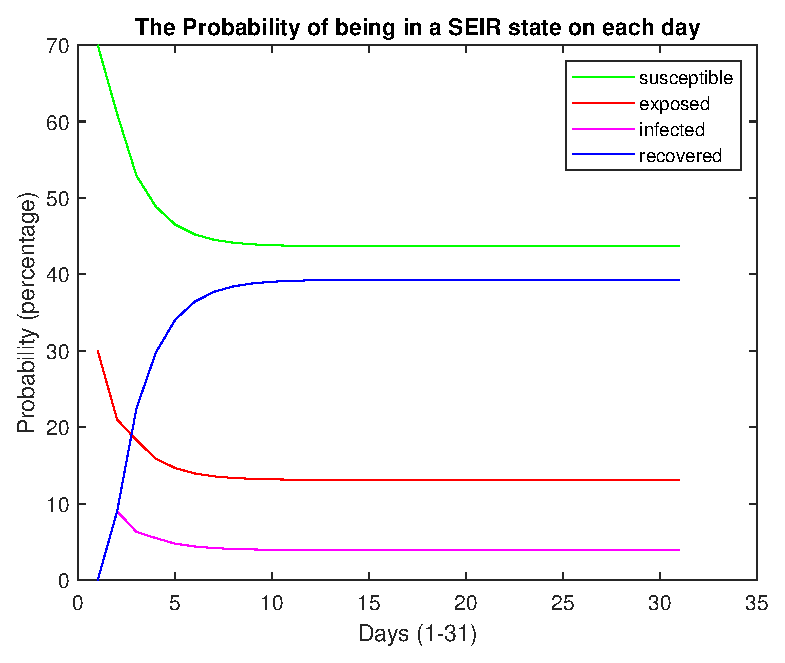
\includegraphics [width=4in]{main_01.eps}


\subsection*{2}

\begin{verbatim}
%(a)
susceptible_2 = [0.15; 0.85; 0; 0];
days_2 = 1:1:31;
prob_day_2 = zeros(4, 1);
prob_s_2 = zeros(1, 31);
prob_e_2 = zeros(1, 31);
prob_i_2 = zeros(1, 31);
prob_r_2 = zeros(1, 31);


for n = 1:31
    prob_day_2 = (transition_SEIR ^ n) * susceptible_2;
    prob_day_2 = prob_day_2 / sum(prob_day_2);

    prob_s_2(n) = prob_day_2(1);
    prob_e_2(n) = prob_day_2(2);
    prob_i_2(n) = prob_day_2(3);
    prob_r_2(n) = prob_day_2(4);
end

figure(2);
plot(days, 100*prob_s_2, '-g');
hold on
plot(days, 100*prob_e_2, '-r');
plot(days, 100*prob_i_2, '-m');
plot(days, 100*prob_r_2, '-b');
legend('susceptible', 'exposed', 'infected', 'recovered');
title('The Probability of being in a SEIR state on each day');
xlabel('Days (1-31)');
ylabel('Probability (percentage)');

% (b)
stat_dist_2 = zeros(4, 1);
stat_dist_2(1) = prob_s_2(31);
stat_dist_2(2) = prob_e_2(31);
stat_dist_2(3) = prob_i_2(31);
stat_dist_2(4) = prob_r_2(31);

fprintf('\n\n');
fprintf('The stationary distribution is:\n\n'); disp(stat_dist);
\end{verbatim}

        \color{lightgray} \begin{verbatim}

The stationary distribution is:

    0.4367
    0.1310
    0.0393
    0.3930

\end{verbatim} \color{black}
    
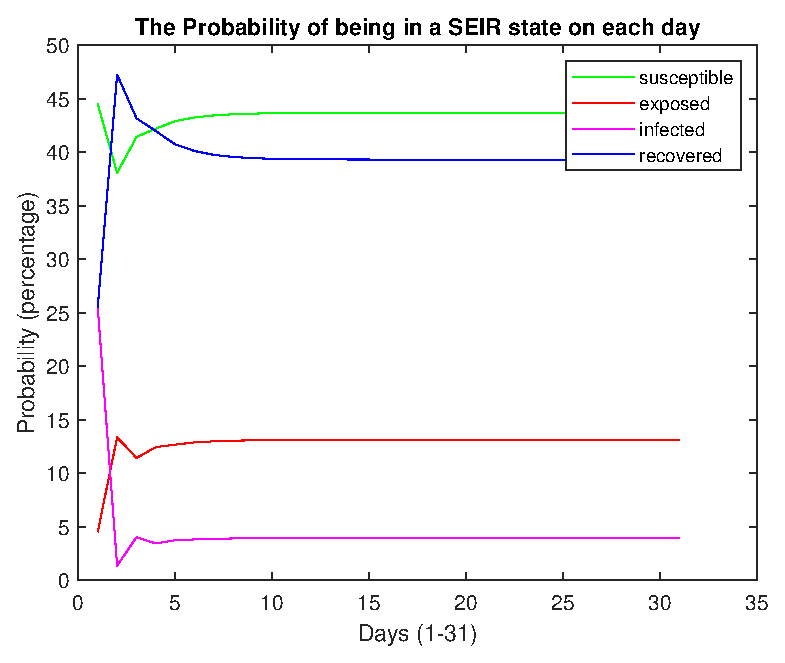
\includegraphics [width=4in]{main_02.eps}


\subsection*{4}

\begin{verbatim}
% lots of math: x_inf = c1v1...

[V, d] = eig(transition_SEIR);

lambdas = [d(1); d(6); d(11); d(16)];
eig_vec_i = V(1:4, 3);

x0_1 = [1; 0; 0; 0];
x0_2 = [0.15; 0.85; 0; 0];

c_1 = V \ x0_1;
c_2 = V \ x0_2;

c_i = c_1(3);
c_i_2 = c_2(3);

disp('Checking that the constant c is the same for initial conditions:');
disp('c_i:'); disp(c_i); disp('c_i_2'); disp(c_i_2);

%eig_vec_i = eig_vec_i / sum(eig_vec_i);

x_inf = c_i * eig_vec_i;
disp(x_inf);

abs_error = zeros(4, 31);
days_4 = 1:1:31;
prob_day_4 = zeros(4, 1);
abs_err_s = zeros(1, 31);
abs_err_e = zeros(1, 31);
abs_err_i = zeros(1, 31);
abs_err_r = zeros(1, 31);


for n = 1:31
    prob_day_4 = (transition_SEIR ^ n) * x0_2;
    prob_day_4 = prob_day_4 / sum(prob_day_4);

    abs_error(1:4, n) = abs(x_inf - prob_day_4);

    abs_err_s(n) = abs_error(1, n);
    abs_err_e(n) = abs_error(2, n);
    abs_err_i(n) = abs_error(3, n);
    abs_err_r(n) = abs_error(4, n);
end

figure(3);
semilogy(days_4, 100*abs_err_s);
hold on
semilogy(days_4, 100*abs_err_e);
semilogy(days_4, 100*abs_err_i);
semilogy(days_4, 100*abs_err_r);
legend('Error Susceptability', 'Error Exposure', 'Error Infection', 'Error Recovered');
title('Absolute Error for Each Step');
xlabel('days (1-31)');
ylabel('absolute error (log scale)');
\end{verbatim}

        \color{lightgray} \begin{verbatim}Checking that the constant c is the same for initial conditions:
c_i:
    0.6032

c_i_2
    0.6032

    0.4367
    0.1310
    0.0393
    0.3930

\end{verbatim} \color{black}
    
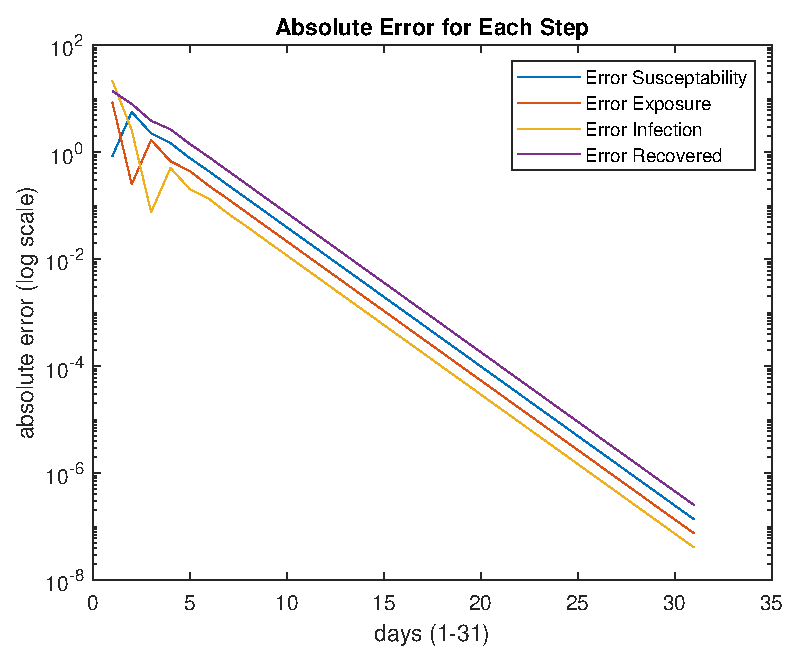
\includegraphics [width=4in]{main_03.eps}


\subsection*{5}

\begin{verbatim}
% (b)
Pim = 1;

transition_SEIR_Im = [Ps, Pe, 0, (1/2)*(1-Pr), 0;
                   1-Ps, 0, 0, 0, 0;
                   0, 1/2*(1-Pe), (1-Pi), 0, 0;
                   0, 1/2*(1-Pe), Pi, Pr, 0;
                   0, 0, 0, (1/2)*(1-Pr), Pim];

fprintf('\n\n');
fprintf('The transistion matrix for the Markov Chain of the SEIR-Im model:\n\n'); disp(transition_SEIR_Im);

% (c)
susceptible_new = [1; 0; 0; 0; 0];
days_3 = 1:1:250;
prob_day_3 = zeros(5, 1);
prob_s_3 = zeros(1, 250);
prob_e_3 = zeros(1, 250);
prob_i_3 = zeros(1, 250);
prob_r_3 = zeros(1, 250);
prob_im = zeros(1, 250);


for n = 1:250
    prob_day_3 = (transition_SEIR_Im ^ n) * susceptible_new;
    prob_day_3 = prob_day_3 / sum(prob_day_3);

    prob_s_3(n) = prob_day_3(1);
    prob_e_3(n) = prob_day_3(2);
    prob_i_3(n) = prob_day_3(3);
    prob_r_3(n) = prob_day_3(4);
    prob_im(n) = prob_day_3(5);
end

figure(4);
plot(days_3, 100*prob_s_3, '-g');
hold on
plot(days_3, 100*prob_e_3, '-r');
plot(days_3, 100*prob_i_3, '-m');
plot(days_3, 100*prob_r_3, '-b');
plot(days_3, 100*prob_im, '-c');
legend('susceptible', 'exposed', 'infected', 'recovered', 'immune');
title('The Probability of being in a SEIR-Im state on each day');
xlabel('Days (1-250)');
ylabel('Probability (percentage)');

stat_dist_3 = zeros(5, 1);
stat_dist_3(1) = prob_s_3(250);
stat_dist_3(2) = prob_e_3(250);
stat_dist_3(3) = prob_i_3(250);
stat_dist_3(4) = prob_r_3(250);
stat_dist_3(5) = prob_im(250);

fprintf('\n\n');
fprintf('The stationary distribution is:\n\n'); disp(stat_dist_3);
\end{verbatim}

        \color{lightgray} \begin{verbatim}

The transistion matrix for the Markov Chain of the SEIR-Im model:

    0.7000    0.4000         0    0.1000         0
    0.3000         0         0         0         0
         0    0.3000         0         0         0
         0    0.3000    1.0000    0.8000         0
         0         0         0    0.1000    1.0000



The stationary distribution is:

    0.0000
    0.0000
    0.0000
    0.0000
    1.0000

\end{verbatim} \color{black}
    
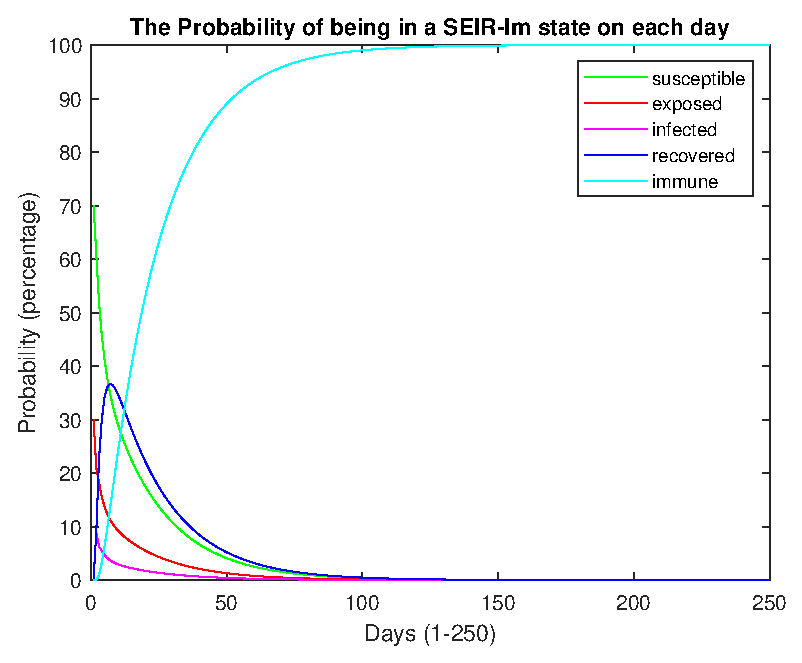
\includegraphics [width=4in]{main_04.eps}


\subsection*{4.1 questions}



\subsection*{1}

\begin{verbatim}
Pex = 0.5;
Pv = 0.25;
Pimu = 1;

transition_SEIR_VIm = [Ps, 0, 0, 1-Pr, 0, 0;
                       1-Ps, 0, 0, 0, 0, 0;
                       0, Pex, 0, 0, 0, 0;
                       0, Pex, Pim, Pr, 0, 0;
                       0, 0, 0, 0,  Pv, 0;
                       0, 0, 0, 0, 1-Pv, Pimu];

fprintf('\n\n');
fprintf('The transistion matrix for the Markov Chain of the SEIR-VIm model:\n\n'); disp(transition_SEIR_VIm);
\end{verbatim}

        \color{lightgray} \begin{verbatim}

The transistion matrix for the Markov Chain of the SEIR-VIm model:

    0.7000         0         0    0.2000         0         0
    0.3000         0         0         0         0         0
         0    0.5000         0         0         0         0
         0    0.5000    1.0000    0.8000         0         0
         0         0         0         0    0.2500         0
         0         0         0         0    0.7500    1.0000

\end{verbatim} \color{black}
    

\subsection*{2}

\begin{verbatim}
[Vnew, dnew] = eig(transition_SEIR_VIm);

lambdasnew = [dnew(1); dnew(8); dnew(15); dnew(22); dnew(29); dnew(36)];
mult1 = 0;
for n = 1:6
    if lambdasnew(n) == 1
        mult1 = mult1 + 1;
    end
end

fprintf('\n\n');
fprintf('The eigenvalue 1 has multiplicity of:'); disp(mult1);
fprintf('\n');
fprintf('This implies that there are two unique stationary distributions.');
fprintf('\n');
% not craystal clear on the 'structural features they are talking about'
fprintf('This is accounted for in the fact the last two columns of the tranisition matirx are independent from the first four.');
\end{verbatim}

        \color{lightgray} \begin{verbatim}

The eigenvalue 1 has multiplicity of:     2


This implies that there are two unique stationary distributions.
This is accounted for in the fact the last two columns of the tranisition matirx are independent from the first four.\end{verbatim} \color{black}
    

\subsection*{3}

\begin{verbatim}
suceptible_5 = [1; 0; 0; 0; 0; 0];
prob_day_5 = zeros(6, 1);
prob_s_5 = zeros(1, 31);
prob_e_5 = zeros(1, 31);
prob_i_5 = zeros(1, 31);
prob_r_5 = zeros(1, 31);
prob_v_5 = zeros(1, 31);
prob_im_5 = zeros(1, 31);


for n = 1:31
    prob_day_5 = (transition_SEIR_VIm ^ n) * suceptible_5;
    prob_day_5 = prob_day_5 / sum(prob_day_5);

    prob_s_5(n) = prob_day_5(1);
    prob_e_5(n) = prob_day_5(2);
    prob_i_5(n) = prob_day_5(3);
    prob_r_5(n) = prob_day_5(4);
    prob_v_5(n) = prob_day_5(5);
    prob_im_5(n) = prob_day_5(6);
end

figure(5);
plot(days, 100*prob_s_5, '-g');
hold on
plot(days, 100*prob_e_5, '-r');
plot(days, 100*prob_i_5, '-m');
plot(days, 100*prob_r_5, '-b');
plot(days, 100*prob_v_5, '-c');
plot(days, 100*prob_im_5, '--k');
legend('susceptible', 'exposed', 'infected', 'recovered', 'vaccinated','immune');
title('The Probability of being in a SEIR-VIm state on each day');
xlabel('Days (1-31)');
ylabel('Probability (percentage)');

% stationary distribution
stat_dist_5 = zeros(6, 1);
stat_dist_5(1) = prob_s_5(31);
stat_dist_5(2) = prob_e_5(31);
stat_dist_5(3) = prob_i_5(31);
stat_dist_5(4) = prob_r_5(31);
stat_dist_5(5) = prob_v_5(31);
stat_dist_5(6) = prob_im_5(31);

fprintf('\n\n');
fprintf('The stationary distribution is:\n\n'); disp(stat_dist_3);
\end{verbatim}

        \color{lightgray} \begin{verbatim}

The stationary distribution is:

    0.0000
    0.0000
    0.0000
    0.0000
    1.0000

\end{verbatim} \color{black}
    
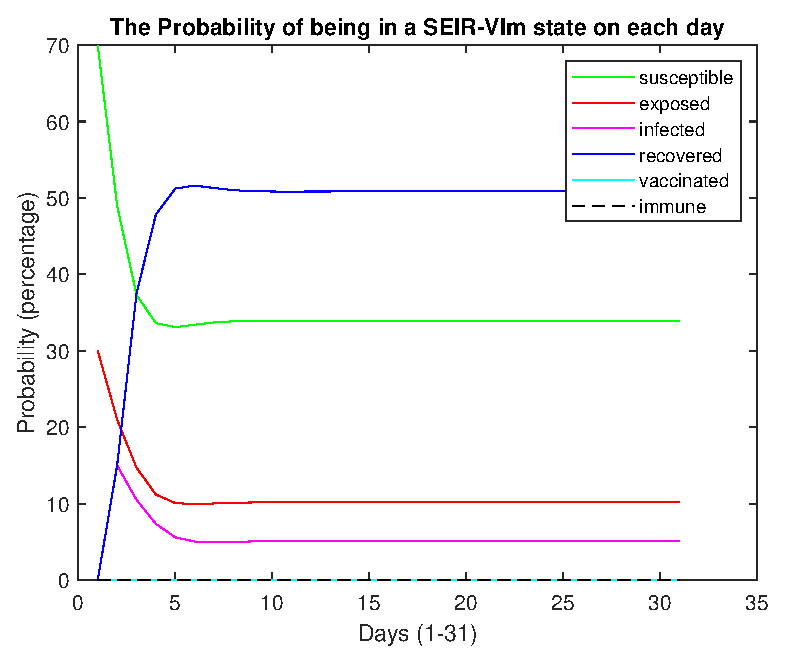
\includegraphics [width=4in]{main_05.eps}


\subsection*{4}

\begin{verbatim}
suceptible_6 = [.33; 0; 0; 0; .67; 0];
prob_day_6 = zeros(6, 1);
prob_s_6 = zeros(1, 31);
prob_e_6 = zeros(1, 31);
prob_i_6 = zeros(1, 31);
prob_r_6 = zeros(1, 31);
prob_v_6 = zeros(1, 31);
prob_im_6 = zeros(1, 31);


for n = 1:31
    prob_day_6 = (transition_SEIR_VIm ^ n) * suceptible_6;
    prob_day_6 = prob_day_6 / sum(prob_day_6);

    prob_s_6(n) = prob_day_6(1);
    prob_e_6(n) = prob_day_6(2);
    prob_i_6(n) = prob_day_6(3);
    prob_r_6(n) = prob_day_6(4);
    prob_v_6(n) = prob_day_6(5);
    prob_im_6(n) = prob_day_6(6);
end

figure(6);
plot(days, 100*prob_s_6, '-g');
hold on
plot(days, 100*prob_e_6, '-r');
plot(days, 100*prob_i_6, '-m');
plot(days, 100*prob_r_6, '-b');
plot(days, 100*prob_v_6, '-c');
plot(days, 100*prob_im_6, '-k');
legend('susceptible', 'exposed', 'infected', 'recovered', 'vaccinated','immune');
title('The Probability of being in a SEIR-VIm state on each day');
xlabel('Days (1-31)');
ylabel('Probability');

% stationary distribution
stat_dist_6 = zeros(6, 1);
stat_dist_6(1) = prob_s_6(31);
stat_dist_6(2) = prob_e_6(31);
stat_dist_6(3) = prob_i_6(31);
stat_dist_6(4) = prob_r_6(31);
stat_dist_6(5) = prob_v_6(31);
stat_dist_6(6) = prob_im_6(31);

fprintf('\n\n');
fprintf('The stationary distribution is:\n\n'); disp(stat_dist_6);
\end{verbatim}

        \color{lightgray} \begin{verbatim}

The stationary distribution is:

    0.1119
    0.0336
    0.0168
    0.1678
    0.0000
    0.6700

\end{verbatim} \color{black}
    
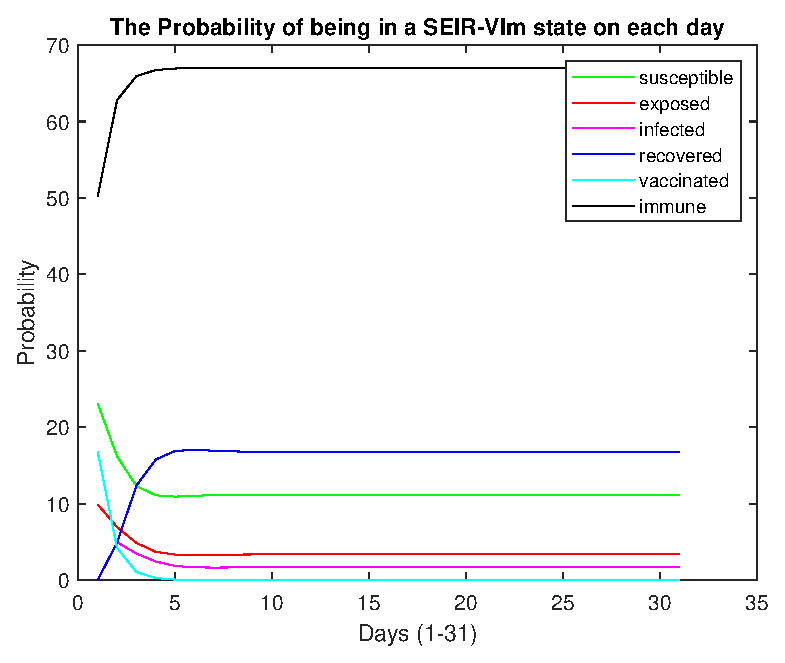
\includegraphics [width=4in]{main_06.eps}


\subsection*{5}

\begin{verbatim}
fprintf('\n\n');
fprintf('In order for the stationary distribution to have any values for vaccinated or immune, the initial state vector has to contaion values for these two categories.');
fprintf('\n\n');
fprintf('In problem 3, there were no non zero initial conditions for vaccinated or immune and therefore, the stationary state graph only had sero values for these two states.');
fprintf('\n\n');
% can only think of the same 'structural feasture' as before...
fprintf('This is accounted for by the fact that the last two columns of the trasition matix do not depend on the first four.');
\end{verbatim}

        \color{lightgray} \begin{verbatim}

In order for the stationary distribution to have any values for vaccinated or immune, the initial state vector has to contaion values for these two categories.

In problem 3, there were no non zero initial conditions for vaccinated or immune and therefore, the stationary state graph only had sero values for these two states.

This is accounted for by the fact that the last two columns of the trasition matix do not depend on the first four.\end{verbatim} \color{black}
    


\end{document}
    
